\selectlanguage{ngerman}%
\frenchspacing%
\begin{ledgroupsized}[r]{120mm}%
\footnotesize%
\pstart%
\noindent%
\textbf{Überlieferung:}%
\pend%
\end{ledgroupsized}%
\begin{ledgroupsized}[r]{114mm}%
\footnotesize%
\pstart%
\parindent -6mm%
\makebox[6mm][l]{\textit{L}}%
Aufzeichnung:
LH XXXV 13,\;2c Bl.\;112--113.
Ein Bogen 2\textsuperscript{o},
Bl.\;113 um die oberen zwei Drittel beschnitten;
Gegenmarke eines Wasserzeichens auf Bl.\;112 mittig. %
Eineinviertel Seiten auf Bl.\;112,
wobei die Zeichnungen in der oberen Hälfte von Bl.\;\href{\Scan{LH_35_13_02c_112r}}{112\,r\textsuperscript{o}} (S.\;\pageref{LH_35_13_02c_112r_zchn}) keinen unmittelbaren Zusammenhang mit N.\;\ref{57960} aufweisen.
Bl.\;\href{\Scan{LH_35_13_02c_113r}}{113\,r\textsuperscript{o}} ist unbeschrieben;
Bl.\;\href{\Scan{LH_35_13_02c_113v}}{113\,v\textsuperscript{o}} überliefert einen mathematischen Text zur Differentialgeometrie, der voraussichtlich in einem künftigen Band von \textit{LSB}\;VII ediert werden wird.%
\pend%
\end{ledgroupsized}%
\vspace{5mm}%
\begin{ledgroup}%
\footnotesize%
\pstart%
\noindent%
\textbf{Datierungsgründe:}
Die Datierung der Aufzeichnung N.\;\ref{57960} beruht auf äußeren Eigenschaften des Texträgers sowie auf inhaltlichen Betrachtungen.
Siehe die ausführliche Begründung auf S.\;\pageref{57960_dat}.%
\pend%
\end{ledgroup}%
\selectlanguage{latin}%
\frenchspacing%
\vspace*{6mm}
\normalsize%
\pstart%
\noindent%
\lbrack%
\href{\Scan{LH_35_13_02c_112r}}%
{112\,r\textsuperscript{o}}%
\rbrack\ %
\edlabel{LH_35_13_02c_112r_bedng-1}%
\edtext{}{%
\xxref{LH_35_13_02c_112r_bedng-1}{LH_35_13_02c_112r_bedng-2}%
\lemma{\textit{AB} cyl. \lbrack...\rbrack\ ad 3}%
\Cfootnote{%
Der Zylinder \textit{LM} hat eine Höhe von 27 Zoll und einen Durchmesser von $\displaystyle\frac{1}{3}$ Zoll (vgl. \refpassage{LH_35_13_02c_112v_masse-1}{LH_35_13_02c_112v_masse-2}).
Sein Volumen wird im Folgenden mit dem eines weiteren Zylinders verglichen, dessen Höhe und Durchmesser die gleiche Länge \textit{AB} aufweisen.
Siehe die Diagramme \lbrack\textit{Fig.\:1}\rbrack\ und \lbrack\textit{Fig.\:2}\rbrack.
}}%
\textit{AB}\;cyl.%
\indexS{cylinder}
est ad cyl.\;%
\edtext{%
\textit{LM},
ut $AB^3$ ad
$27\cdot\displaystyle\frac{1}{9}\;\lbrack=\rbrack\;\displaystyle\frac{27}{9}$,
\lbrack seu\rbrack\
ut $AB^3$ ad 3.%
\edlabel{LH_35_13_02c_112r_bedng-2}%
\newline%
Jam sphaera inscripta%
\indexS{sphaera inscripta cylindro}
est ad cylindrum \textit{AB},
ut~2 ad~3.%
}{%
\lemma{\textit{LM},}%
\Bfootnote{%
ut $AB^3$ ad
\bars{$27 \cdot \displaystyle\frac{1}{9} \cdot \displaystyle\frac{27}{9}$, \textit{ändert Hrsg.}} 
ut $AB^3$ %
\textit{(1)}~ad %
\textit{(2)}~ad %
\textit{(a)}~$\displaystyle\frac{1}{3}$ %
\textit{(b)}~3. %
\textit{(aa)}~Ergo cylinder \textit{AB} %
\textit{(bb)}~$\displaystyle\frac{2}{9}$. Er %
\textit{(cc)}~Ergo cylinder \textit{AB} est ad cylind %
\textit{(dd)}~Jam sphaera %
\lbrack...\rbrack\ \textit{AB}, ut %
\bars{ut \textit{ streicht Hrsg.}} 2 ad~3.%
~\textit{L}%
}}
\rule[0mm]{0pt}{4.3mm}%
\edtext{%
Ergo sphaera inscripta est ad cylind.\;\textit{LM}
\rule[0mm]{0pt}{5.8mm}%
ut~2 ad~1.%
}{%
\lemma{Ergo \lbrack...\rbrack\ 2~ad~1}%
\Cfootnote{%
Unter den angegebenen Bedingungen (\refpassage{LH_35_13_02c_112r_bedng-1}{LH_35_13_02c_112r_bedng-2}) verhält sich das Volumen der vom Zylinder \textit{AB} umbeschriebenen Kugel zum Volumen des Zylinders \textit{LM} wie $\displaystyle\frac{2}{3}AB^3$ zu 3 Zoll\textsuperscript{3}.
}}
\pend%
\pstart%
\noindent%
Cyl.\;\textit{LM}%
\indexS{cylinder}
\edlabel{lh035_13_2c_112r_1a}%
ad cyl.\;\textit{AB}%
\edtext{}{%
\xxref{lh035_13_2c_112r_1a}{lh035_13_2c_112r_1b}%
\lemma{ad cyl.\;\textit{AB}}%
\Bfootnote{%
\textit{(1)}~ut %
\textit{(a)}~\textit{A} %
\textit{(b)}~$3\cdot AB^3$ ad %
\textit{(2)}~ut 3 %
\textit{(a)}~$\displaystyle\frac{1}{3}$ %
\textit{(b)}~ad $AB^3$ %
\textit{(aa)}~vel ut ad $3AB^3$ cyl. %
\textit{(aaa)}~$AB^3$ %
\textit{(bbb)}~\textit{AB} ad %
\textit{(bb)}~. Ergo cyl. $AB = \text{cyl.}\ \displaystyle\frac{LM\ \text{per}\ AB^3}{3}$. %
\textit{(aaa)}~Ergo cyl.\;$AB = 3 \cdot \text{cyl.}\;LM\ \text{per}\ AB^3$ %
\textit{(bbb)}~Jam sphaerae %
\lbrack...\rbrack\ cylind. \textit{AB} %
\bars{inscr. \textit{erg.}} valor est %
\bars{$\displaystyle\frac{2 \cdot\ \text{cyl.}\;LM\ \text{per}\ A^3B^3}{3}$ \textit{ändert Hrsg.}}.%
~\textit{L}%
}}
ut 3 ad $AB^3$. %
Ergo cyl.\;%
\rule[0mm]{0pt}{6.2mm}%
$AB = \displaystyle\frac{\text{cyl.}\; LM\ \text{per}\ AB^3}{3}$.
\newline%
Jam sphaerae
cylindro \textit{AB} inscriptae%
\indexS{sphaera inscripta cylindro}%
\indexS{cylinder}
valor est%
\indexS{valor}
$\displaystyle\frac{2}{3}$ cylind.\;\textit{AB}.
Ergo sphaerae cylind.\;\textit{AB} inscr.
valor est $\displaystyle\frac{2\cdot\text{cyl.}\ LM\ \text{per}\ AB^3}{[9]}$.%
\indexS{sphaera inscripta cylindro}%
\indexS{cylinder}%
\indexS{valor}%
\edlabel{lh035_13_2c_112r_1b}
\pend%
\newpage%
\begin{edfigure}[0em][2.5em]%
\hspace{-44mm}%
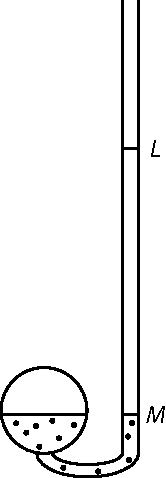
\includegraphics[width=0.18\textwidth]{gesamttex/edit_VIII-4/images/LH_35_13_02c_112-113_d1_112r.pdf}
\edcaption[1.0em]%
{%
\hspace*{-44mm}%
\lbrack\textit{Fig.\:1}\rbrack%
}%
\vspace{-11.9em}%
\hspace{44mm}%
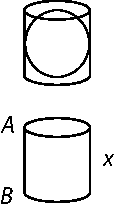
\includegraphics[width=0.136\textwidth]{gesamttex/edit_VIII-4/images/LH_35_13_02c_112-113_d2_112r.pdf}
\edcaption[1.0em]%
{%
\hspace*{44mm}%
\lbrack\textit{Fig.\:2}\rbrack%
}%
\end{edfigure}%
\pstart%
\noindent%
\edtext{%
Sphaer. \astrosun\ $ = 2\ \text{pl.\;cyl.}\ LM$.
Ergo sphaer. cyl.\;\textit{AB} inscr. valor est
$\displaystyle\frac{\text{sphaer. \astrosun}\ \text{per}\ AB^3}{[9]}$.%
\indexS{sphaera inscripta cylindro}%
\indexS{cylinder}%
\indexS{valor}%
}{%
\lemma{Sphaer. \astrosun\ $ = 2\ \text{pl.\;cyl.}\ LM$.}%
\Bfootnote{%
\textit{(1)}~Ergo cyl. $LM = \displaystyle\frac{1}{2} \cdot \text{sphaer.}\ \astrosun$ %
\textit{(2)}~Ergo sphaer. %
\lbrack...\rbrack\ valor est %
\bars{$\displaystyle\frac{\text{sphaer. \astrosun}\ \text{per}\ AB^3}{3}$ \textit{ändert Hrsg.}}.%
~\textit{L}%
}}
\pend%
\pstart%
\noindent%
Jam sphaerae sunt ut cubi diam.%
\indexS{cubus diametri}%
\rule[0mm]{0pt}{3.6mm}
Sphaer.\;\astrosun\ diameter sit \textit{x}.
Sphaerae cyl.\;\textit{AB}
inscriptae diameter %
est \textit{AB}.%
\indexS{sphaera inscripta cylindro}%
\indexS{cylinder}%
\indexS{diameter sphaerae}
Ergo sphaer. \astrosun\ ad sphaer. \textit{AB}
ut $x^3$
\edtext{%
ad $AB^3$.
\newline%
\edtext{%
Jam supra
sph. \astrosun\ est ad sph.\;\textit{AB}
ut $AB^3$ ad~3.%
\indexS{sphaera inscripta cylindro}%
}{%
\lemma{Jam \lbrack...\rbrack\ ad~3}%
\Cfootnote{%
Das Verhältnis zwischen den Kugeln entspricht dem Verhältnis zwischen den jeweiligen Zylindern;
vgl. \refpassage{LH_35_13_02c_112r_bedng-1}{LH_35_13_02c_112r_bedng-2}.%
}}%
}{%
\lemma{ad $AB^3$.}%
\Bfootnote{%
\textit{(1)}~Ergo sphaer$AB = \text{sphaer}\ \astrosun \cdot\ AB^3 : x^3$. %
\textit{(2)}~Jam supra %
\lbrack...\rbrack\ $AB^3$ ad 3.%
~\textit{L}%
}}
Ergo $x^3$ est ad $AB^3$
ut $AB^3$ ad 3,
vel $x^3 = AB^6 : 3$,
vel
$x = AB^2 :
\edtext{%
\lbrack\sqrt[3]{3}\rbrack$.%
}{%
\lemma{$\surd{3}$}%
\Bfootnote{%
\textit{L\;ändert Hrsg.}%
}}
\lbrack%
\href{\Scan{LH_35_13_02c_112v}}%
{112\,v\textsuperscript{o}}%
\rbrack%
\pend%
\vspace{1.0em}%
\pstart%
\noindent%
\edlabel{LH_35_13_02c_112v_masse-1}%
\textit{LM} 27 Zoll hoch,%
\indexS{Zoll}
weit $\displaystyle\frac{1}{3}$ Zoll,%
\edlabel{LH_35_13_02c_112v_masse-2}
thut am
\lbrack\textit{Text bricht ab.}\rbrack%
\pend%
\newpage%
\begin{edfigure}[0em][4.0em]%
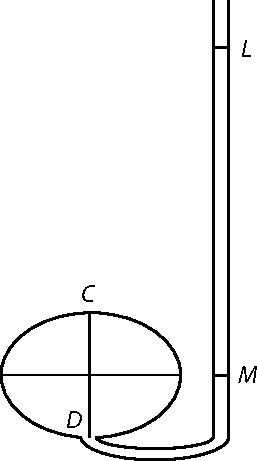
\includegraphics[width=0.26\textwidth]{gesamttex/edit_VIII-4/images/LH_35_13_02c_112-113_d3_112v.pdf}
\edcaption[0.750em]%
{%
\lbrack\textit{Fig.\:3}\rbrack%
}%
\end{edfigure}%
\pstart%
\noindent%
\pagelabel{LH_35_13_02c_112r_zchn}%
\lbrack%
\textit{Auf Bl.\;\href{\Scan{LH_35_13_02c_112r}}{112\,r\textsuperscript{o}}, ohne erkennbaren Zusammenhang mit N.\;\ref{57960}:}%
\rbrack%
\pend%
\begin{edfigure}[2.5em][0.0em]%
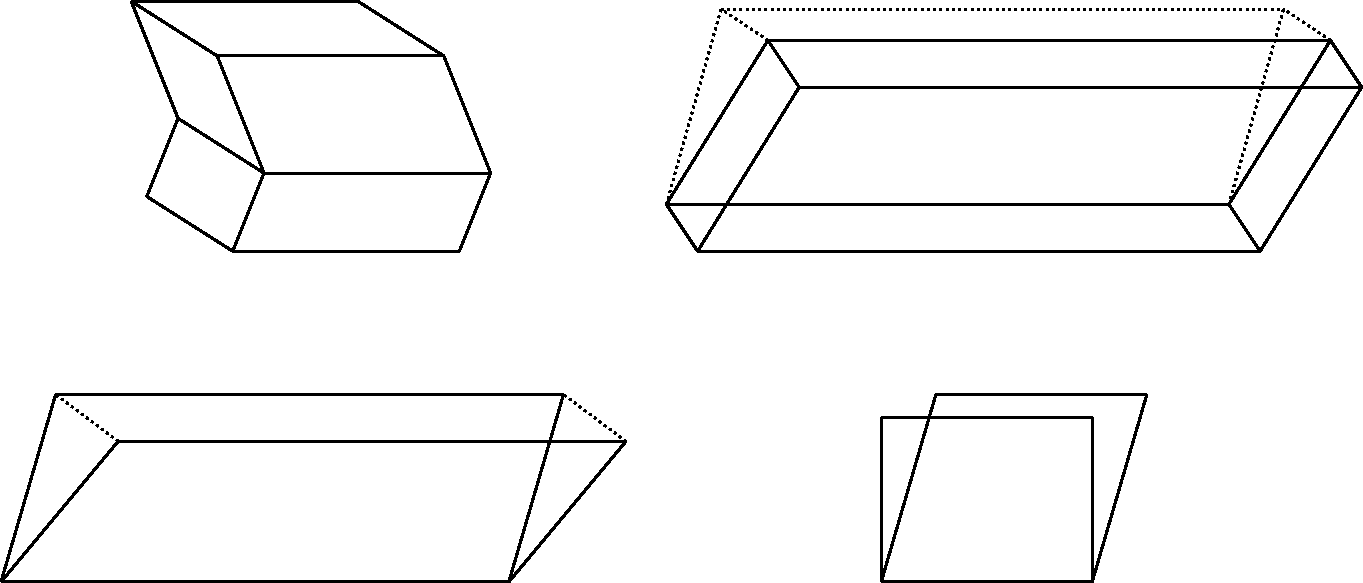
\includegraphics[width=0.72\textwidth]{gesamttex/edit_VIII-4/images/LH_35_13_02c_112-113_d4_112r.pdf}
\edcaption[1.0em]%
{%
\lbrack\textit{Fig.\:4}\rbrack%
}%
\end{edfigure}%
\newpage%
\vspace{4.0em}%
\pstart%
\noindent%
\centering%
*     *     *
\pend%
\vspace{2.0em}%
\selectlanguage{german}%
\frenchspacing%
\footnotesize%
\pstart%
\noindent%
\textls{Ausführliche Datierungsgründe:}%
\pagelabel{57960_dat}
In der titellosen und undatierten Aufzeichnung N.\;\ref{57960}, die einen eher flüchtigen Charakter aufweist, versucht Leibniz, von einem 27 Zoll langen und 1/3 Zoll weiten Rohr ausgehend, eine von einem Zylinder gleichen Volumens umbeschriebene Kugel zu bestimmen.
Rohr und Kugel sind offenbar, wie auch die Diagramme \lbrack\textit{Fig.\:1}\rbrack\ und \lbrack\textit{Fig.\:3}\rbrack\ nahelegen, als Teile eines Barometers zu verstehen.
Die Aufzeichnung N.\;\ref{57960} dürfte somit im Zusammenhang mit Überlegungen über die Beschaffenheit oder den Aufbau eines Barometers entstanden sein.
\pend%
\pstart%
Im Textträger ist die Gegenmarke eines Wasserzeichens anzutreffen, das im Leibniz-Nachlass %
nach heutigem Wissensstand für einen Zeitraum belegt ist, der sich von der frühen Hannoveraner\indexO{Hannover} Zeit bis in die zweite Hälfte der 1690er Jahre erstreckt.
Die Datierung von N.\;\ref{57960} lässt sich möglicherweise aber anhand der Beobachtung einschränken, dass die meisten Überlegungen, die Leibniz der Beschaffenheit oder dem Aufbau des Barometers gewidmet hat, vom Herbst 1677 stammen; siehe die im vorliegenden Band unter N.\;\ref{barom-portab_intro}, N.\;\ref{55813-E} und N.\;\ref{motus-perpetuus_intro} veröffentlichten Aufzeichnungen.
N.\;\ref{57960} könnte insbesondere in Zusammenhang mit Leibnizens Überlegungen über ein tragbares Barometer in N.\;\ref{barom-portab_intro} (August – 12./22.\;November 1677) entstanden sein.
Unter dieser Annahme könnte N.\;\ref{57960} ebenfalls im Herbst 1677 verfasst worden sein.
Eine frühere oder eine spätere Datierung sind aber ohne Weiteres möglich.
\pend%
\selectlanguage{latin}%
\frenchspacing%
\normalsize%
\newpage%
